Pour pouvoir poursuivre le développement du site, il est nécessaire d’installer Django (et par conséquent python). Pour ce faire, il est conseillé de suivre le guide d’installation rapide disponible à l’adresse suivante : \href{https://docs.djangoproject.com/fr/1.8/intro/install/}{https://docs.djangoproject.com/fr/1.8/intro/install/}\\

Afin de pouvoir lancer et utiliser le site dans les meilleures conditions possibles, il est nécessaire d’installer plusieurs librairies. Pour ce faire, il suffit d’ouvrir le terminal et de lancer les commandes suivantes :\\
\begin{itemize}
\item pip install splinter
\item pip install geocoder
\item pip install reportlab
\item pip install sendgrid-django
\item pip install selenium\\
\end{itemize}

Si vous rencontrez certains problèmes au niveau des permissions pour exécuter les commandes ci-dessus, il est possible de les exécuter avec un argument supplémentaire --user. Exemple :\\
\begin{itemize}
\item pip install --user splinter\\
\end{itemize}

Il vous est désormais possible de lancer le site en version locale en vous rendant, via le terminal, dans le dossier "ASMAE" et en entrant la commande suivante :\\
\begin{itemize}
\item python manage.py runserve\\
\end{itemize}

\begin{figure}[H]
\centering
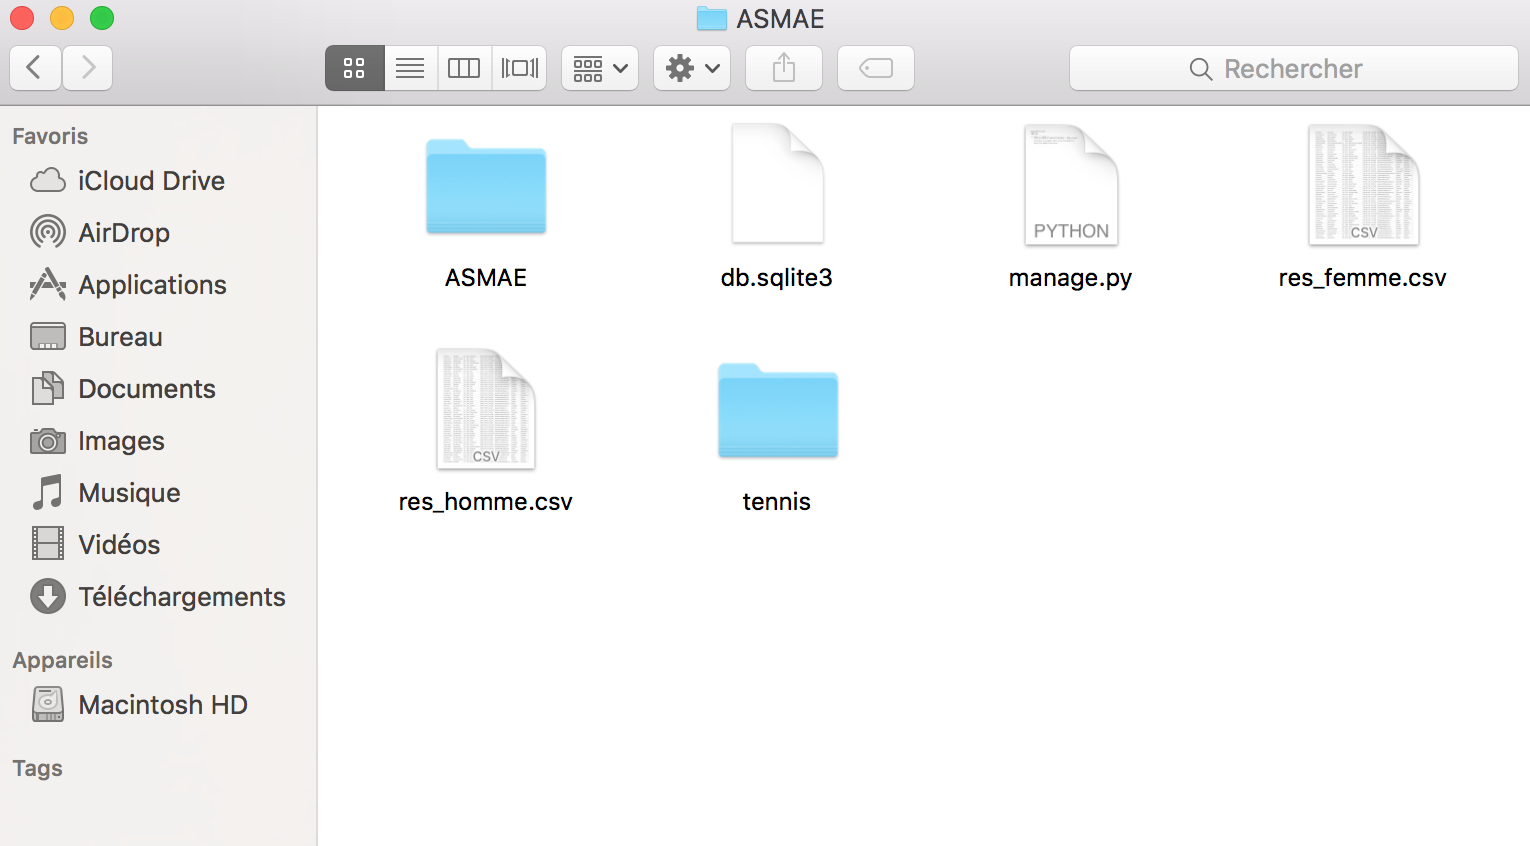
\includegraphics[scale=0.35]{repertory.png}
\caption{Dossier ASMAE}
\end{figure}

Il suffit ensuite de lancer le navigateur de votre choix et de vous rendre à l’adresse suivante : \href{http://localhost:8000/}{http://localhost:8000/}

\begin{figure}[H]
\centering
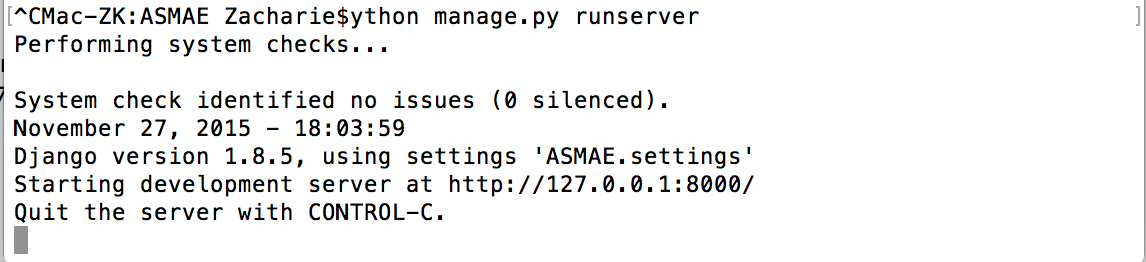
\includegraphics[scale=0.7]{terminal.png}
\caption{Réponse du serveur dans le terminal}
\end{figure}